\documentclass[a4paper,12pt]{report}    % Document Class
% % % % % % % % % % % % % % % % % % % % % % % % % % % % % % % % %
% % % % PACKAGES
% % % % % % % % % % % % % % % % % % % % % % % % % % % % % % % % %
\linespread{1.5}                    % For line spacing
\usepackage{amssymb}                % For AMS symbol
\usepackage{amsmath}                % This is useful for the matrix 
\usepackage{verbatim}               % For comments in paragraph
\usepackage{graphicx}               % For imbeding graph
\usepackage{color}                  % Color for the text
\usepackage{makeidx}
\usepackage{url}
%\usepackage{apacite}
\usepackage{sectsty}
\chapterfont{\centering}



% % % % % % % % % % % % % % % % % % % % % % %
% % % % FOR ADJUSTMENT OF PAGES
% % % % % % % % % % % % % % % % % % % % % % %
\usepackage[top=2cm, bottom=2cm, left=3cm, right=2cm]{geometry}

% % % % % % % % % % % % % % % % % % % % % % % %
% % % % FOR SHORTCUT USE
% % % % % % % % % % % % % % % % % % % % % % % %
\newtheorem{df}{Definition} % For definition
\newtheorem{exm}{Example}   % For Example
\newtheorem{exe}{Exercise}  % For Exercise
\newtheorem{prob}{Problem}  % For Problem
\newtheorem{task}{TASK}     % For Task
\newtheorem{thm}{Theorem}   % For Theorem
% % % % % % % % % % % % % % % % % % % % % % % % %
\renewcommand{\chaptername}{CHAPTER}
\renewcommand{\contentsname}{\centering CONTENTS}
\renewcommand{\listfigurename}{\centering LIST OF FIGURES}
\renewcommand{\listtablename}{\centering LIST OF TABLES}

%%%%%%%%%%%%%%%%%%%%%%%%%%%%%%%%%%%%%%%%%%%%%%%%%%%%%%%
\pagestyle{plain}
%==================================================================
\begin{document}
% % % % % % % % % % % % %
\pagenumbering{roman}
%===================================================================
%   Begin your document hereafter
%=====================================================================


{\large
\begin{center}
{{\bf{\color{red}EXPLORATORY DATA ANALYSIS OF GENETIC DATA}}}\\
\end{center}


\vspace{0.8cm}

{\normalsize
\begin{center}
A SECOND YEAR PROJECT REPORT\\

\vspace{0.5cm}
SUBMITTED IN PARTIAL FULFILLMENT OF THE REQUIREMENTS FOR\\
THE DEGREE OF B.Sc. IN COMPUTATIONAL MATHEMATICS\\

\vspace{1.0cm}

BY
\end{center}
\begin{center}
\begin{itemize}
\begin{center}
\item[1.] Aayush Shrestha (21)
\item[2.] Anmol Jha (31)

\end{center}
\end{itemize}

\end{center}


\vspace{1.0cm}

\begin{figure}[htpb]
\centering

\includegraphics[height=4.5cm,width=4.5cm]{photos/kulogo.jpg}
\end{figure}


\vspace{2cm}
{\normalsize
\begin{center}
DEPARTMENT OF MATHEMATICS\\
SCHOOL OF SCIENCE\\
KATHMANDU UNIVERSITY\\
DHULIKHEL, NEPAL\\
\end{center}
}

\begin{center}
	{\color{red} June 2023}
\end{center}

}
}

%\underbrace{}
\thispagestyle{empty}	% No numbering in this page

%===================================================================
%\newpage
%\input{Dedication}

%\newpage
%\input{Student_declaration}

\newpage



%\addcontentsline{toc}{chapter}{\bf Certification}
\addcontentsline{toc}{chapter}{\bf CERTIFICATION}

\begin{center}
	{\Large{\bf{ CERTIFICATION}}}
\end{center}


\noindent
This project entitled Exploratory Data Analysis of Genetic Data is carried out  under my supervision for the specified entire period satisfactorily, and is hereby certified as a work done by following students
\begin{itemize}
\item[1.] Aayush Shrestha (21)
\item[2.] Anmoj Jha (31)
\end{itemize}
 in partial fulfillment of the requirements for the degree of B.Sc. in Computational Mathematics, Department of Natural Sciences, Kathmandu University, Dhulikhel, Nepal.

\vspace{2.0cm}

\noindent
-----------------------------\\
{\bf Mr. Kiran Kumar Shrestha}\\
Department of Natural Sciences (Mathematics),\\
School of Science, Kathmandu University,\\
Dhulikhel, Kavre, Nepal\\
Date:-----------------------------\\

\vspace{2cm}

\noindent
{\bf APPROVED BY:}\\
I hereby declare that the candidate qualifies to submit this  report of the  Math Project (MATH 252) to the Department of Natural Sciences. 



\vspace{2cm}

\noindent
-----------------------------\\
Dr. Rabindra Kayastha\\
Department of Mathematics\\
School of Science\\
Kathmandu University\\
Date:-----------------------------\\
  


\newpage



%\addcontentsline{toc}{chapter}{\bf Acknowledgements}
\addcontentsline{toc}{chapter}{\bf ACKNOWLEDGEMENTS}
%{\Large{\bf{ACKNOWLEDGMENTS}}}\\

\begin{center}
	{\Large{\bf{ACKNOWLEDGMENTS}}}\\
\end{center}


\noindent
This project was carried out under the supervision of Mr. Kiran Kumar Shrestha. I would like to express my sincere gratitude towards my supervisors for his excellent supervision, guidance and suggestion for accomplishing this work. And to the entire faculty of Department of Natural Sciences (Mathematics) for encouraging, supporting and providing this opportunity.\\

\noindent
I am indebted to all my friends for helping and guiding me over the related software. \\

\noindent
Special appreciation goes to Mr. Simon K. Shrestha(Department Of Biotechnology) for his help with the analysis of genetic data and his valuable suggestions. \\


\noindent
Lastly, we would like to thank everyone who helped us directly and indirectly during the duration of completing our project work.





\newpage



%\addcontentsline{toc}{chapter}{\bf Abstract}
\addcontentsline{toc}{chapter}{\bf ABSTRACT}

\begin{center}
	{\Large{\bf{ABSTRACT}}}\\
\end{center}

\noindent
This report summarizes a semester-long effort that looked at medical data through data analysis and the development of an approachable dashboard to display the results.The goal is to extract insightful knowledge from the data and offer decision-supporting tools to healthcare practitioners.\\

\noindent
The project entails preparing and cleaning the data, then using statistical analysis methods. Despite obstacles like missing values, a broad medical data set from recognized healthcare organizations is utilized. Strategies are used to deal with these problems.\\

\noindent
Finding patterns, trends, and relationships in the medical data is one of the anticipated results. The project's goal is to find significant insights that can improve medical procedures and patient care by utilizing the right visualization libraries and statistical approaches. The results will aid in bettering healthcare decision-making.\\

\noindent
Numerous results are expected. First, the study will provide crucial information about demographic trends and correlations between variables. Second, by enabling healthcare practitioners and the concerned patient to make data-driven decisions, the dashboard will streamline procedures and improve productivity in the medical industry.\\

\noindent
To sum up, the purpose of this project is to analyze medical data thoroughly and produce an interactive dashboard that will show the results. \\


% ===================================================================

\tableofcontents


\listoffigures
%\addcontentsline{toc}{chapter}{List of Figures}
\addcontentsline{toc}{chapter}{LIST OF FIGURES}

\listoftables
%\addcontentsline{toc}{chapter}{List of Tables}
\addcontentsline{toc}{chapter}{LIST OF TABLES}

%\newpage
%



%\addcontentsline{toc}{chapter}{\bf List of Symbols}
\addcontentsline{toc}{chapter}{\bf LIST OF SYMBOLS}

\begin{center}
	{\LARGE{\bf{LIST OF SYMBOLS}}}\\
\end{center}


Your parameters here.

% ====================================================================
\newpage
\pagenumbering{arabic}

\chapter{INTRODUCTION}

\section{{\bf{Background}}}

The availability of enormous volumes of data in the healthcare industry in recent years has greatly increased the prospects for understanding and enhancing decision-making. A key tool for identifying patterns, trends, and correlations in large medical datasets is exploratory data analysis (EDA). To visualize these insights and support data-driven decision-making in the healthcare industry, interactive dashboard creation has also become crucial.\\
\noindent
The necessity to use EDA and dashboard generation to solve issues and enhance healthcare procedures is what spurred this project's inception. The sheer volume and complexity of medical data are often too much for traditional analysis tools to manage, making it difficult to draw useful conclusions.Data scientists and healthcare professionals can find hidden patterns, outliers, and correlations in the data by using EDA's systematic and exploratory methodology.\\
\noindent
Additionally, interactive dashboards that visualize these insights are a potent tool for better data communication and decision-making. Healthcare personnel may engage with data visualizations, personalize views, and receive insightful information quickly thanks to dashboards' straightforward and user-friendly interfaces. EDA and dashboard development have the power to transform healthcare procedures, maximize resource use, and improve patient care.


\section{{\bf{Objectives}}}
{The Objectives of this project were as follows
\begin{enumerate}
 \item Familiarity with data cleaning, feature extraction, and data conversion. 
 \item Describing the data using statistical method such as mean, median, standard deviation, correlation and so on. 
 \item Implementation of different plots in R to understand the data better. 
 \item Implementation of a dashboard.
 \item Understanding and explaining the trends and outliers in the data based on the domain.
\end{enumerate}
}

\section{\bf Significance}
Exploratory data analysis (EDA) and the development of interactive dashboards hold the potential to transform healthcare procedures, which is why this initiative is significant. This research intends to identify useful insights, such as correlations, trends, and risk factors that can significantly influence decision-making in the healthcare industry by conducting a thorough EDA on medical data. These insights can aid healthcare practitioners in maximizing resource allocation, enhancing overall health care plans, and improving patient outcomes. A user-friendly platform for visualizing and analyzing these insights will be provided by the creation of an interactive dashboard customized to the requirements of healthcare professionals, enabling users to make defensible decisions based on data-driven evidence.



\section{\bf Limitations}
The data used in this project is synthetic, meaning it has been artificially generated to simulate real-world medical data. Although synthetic data allows for controlled experiments and can provide valuable insights, it may not fully capture the complexity and nuances of actual patient data. The findings and conclusions drawn from the analysis should be interpreted with caution, considering the inherent differences between synthetic and real-world data. Efforts have been made to ensure the quality of synthetic dataset, but there is still a possibility of errors or limitations in the data generation process. The availability of computational resources and time constraints may also impact the scope and depth of the analysis. Despite these limitations, this project serves as an exploration of the potential benefits and challenges associated with synthetic medical data in the context of exploratory data analysis and dashboard creation. It provides insights into the effectiveness of these methodologies and offers considerations for future research utilizing real-world medical data.

\section{\bf Specifications}
-  Language: R (tidy-verse packages, dashboard packages).\\
-  IDE: Jupyter notebook and RStudio\\
-  Dashboard tool: flexboard package and \url{https://visual.is}\\
-  Data: Kaggle dataset\\

\begin{figure}[htpb]
\begin{center}
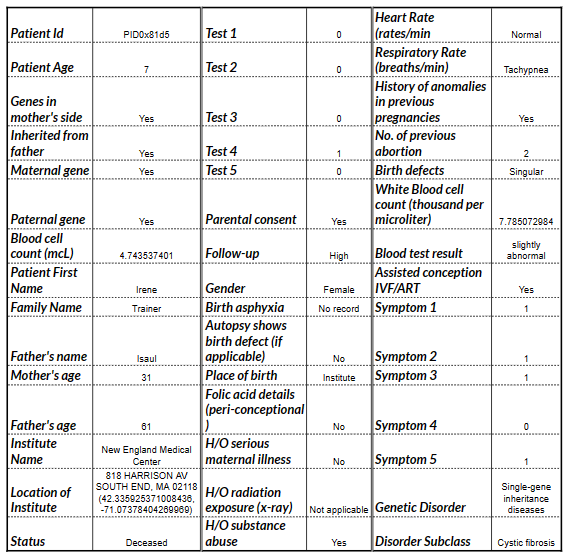
\includegraphics[height=10cm, width=12cm]{figures/sample.png}
\caption{Sample Data Of The Project}
\label{fig 1}
\end{center}
\end{figure}

\newpage

\chapter{METHODOLOGY/MODEL EQUATION}

\section{{\bf{Theoretical/Conceptual Framework}}}
{\bf\color{red}In this section, the author(s) should describe the theoretical/mathematical principles behind the whole work relative to the project. The information collected from literature review shall be relevant in this section.
}


\section{{\bf{Model Equation }}}
Your second section of Section 2 of Chapter 2.
\subsection{\bf Right Aligned Numbering of an Equation}
Your first subsection of Section 2 of Chapter 2.\\
Follow the right aligned numbering of an equation.

\begin{eqnarray}
\rho\,c\,\frac{\partial u}{\partial t} = \nabla \cdot \left( k\, \nabla u \right) + \rho_b\,c_b\,w_b\,(u_a - u) + q_m 
\end{eqnarray}

\subsection{\bf Subsection 2}
Your second subsection of Section 2 of Chapter 2.

\newpage
\chapter{RESULTS}

\section{{\bf{Findings}}}
{\bf In this chapter, we present the results and visualization of the data set and theory described in CHAPTER-2 and finally discuss the results.
}

\section{\bf EDA}
\subsection{Non - Graphical}
Based on summary statistics, there were found columns that had no variance. As such, those columns were removed from the dataset as per the reasoning in 2.3.1 Uni-variate.\\ 

\begin{figure}[htpb]
	\centering
	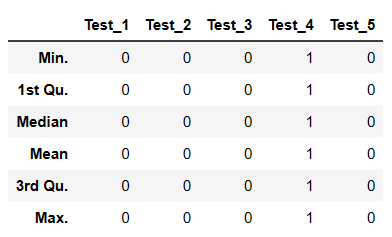
\includegraphics[height=10cm, width=12cm]{figures/s_stat.png}
	\caption{Columns With No Variance}
	\label{fig:columns}
\end{figure}
\noindent
Further more, the following columns were removed based on the domain of study as these columns were deemed to be less significant for further studies of the data. These are:

\begin{table}[htpb]
	\caption{Names Of Discarded Columns}
	\centering
	\begin{tabular}{|c|c|c|}
		\hline
		Patient Id & Patient First Name & Family Name \\
		Father's name & Institute Name  & Location of Institute\\
		Parental consent & Place of birth & H O radiation exposure x.ray\\
		H O substance abuse & & \\
		\hline
	\end{tabular}
	\label{tabl:discarded}
\end{table}

\begin{figure}[htpb]
	\centering
	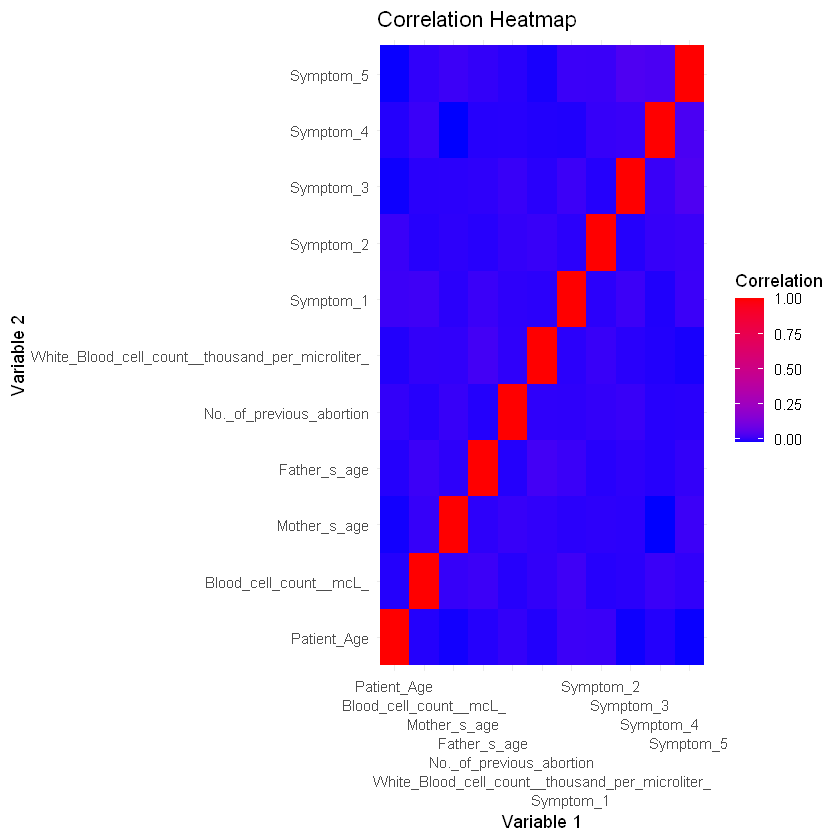
\includegraphics[height=10cm, width=12cm]{figures/corr.png}
	\caption{Correlation Heatmap Of Numeric Attributes}
	\label{fig 3}
\end{figure}

\noindent
Finally, the correlation between every pair of numeric attributes shows that there are no highly correlated attributes.

\newpage
\subsection{Graphical}
Based on the graphical analysis of the attributes in the dataset, we found many columns that does not provide any predictive value with regards to the target attributes.\\
\noindent
According to \cite{han2011data}, attribute significance is an important concept in data mining. The evaluation of attribute usefulness is crucial for effective data analysis. If the distribution of data across different attribute categories is equal, it indicates that the attribute does not have a strong discriminatory power to differentiate between the diseases. This lack of discriminatory power suggests that the test 1 attribute is not significantly associated with the diseases in your dataset.\\
\noindent
Similarly, \cite{mitchell1997machine} discusses the significance of attributes in machine learning. When the distribution of data is symmetric between different attribute categories, it implies that the attribute does not provide valuable predictive information for distinguishing between diseases. In this case, the symmetric distribution of data for the test 1 attribute suggests a lack of significance in relation to the diseases.\\

\begin{figure}[htpb]
	\centering
	\includegraphics[height=10cm, width=12cm]{figures/Status.png}
	\caption{Disorder And Status}
	\label{fig 4}
\end{figure}

\begin{figure}[htpb]
	\centering
	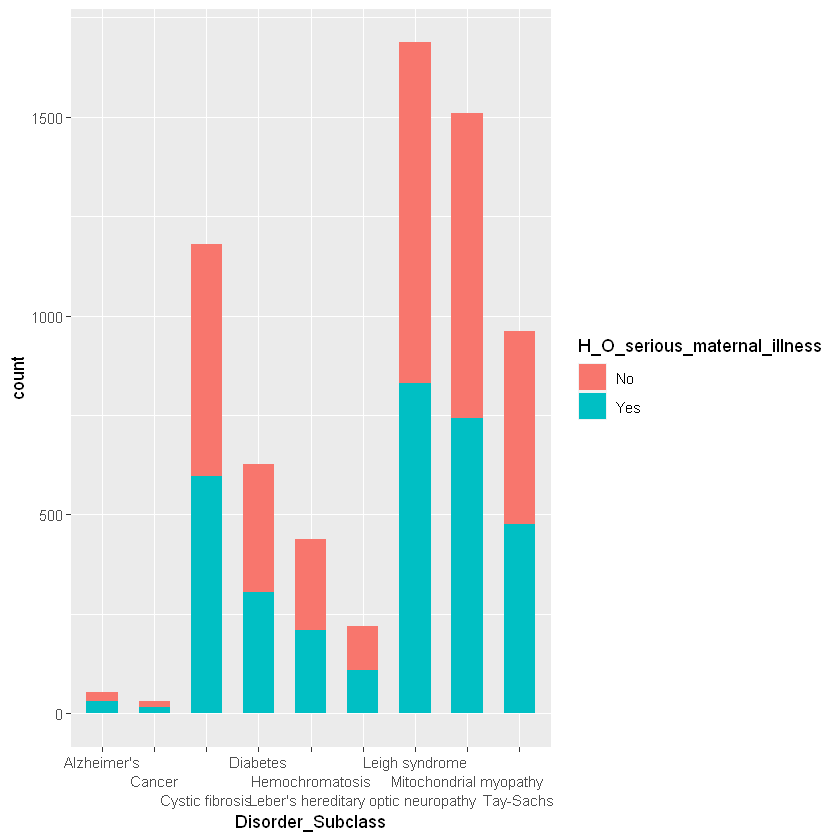
\includegraphics[height=10cm, width=12cm]{figures/maternalill.png}
	\caption{Disorder And History Of Maternal Illness}
	\label{fig 5}
\end{figure}

\begin{figure}[htpb]
	\centering
	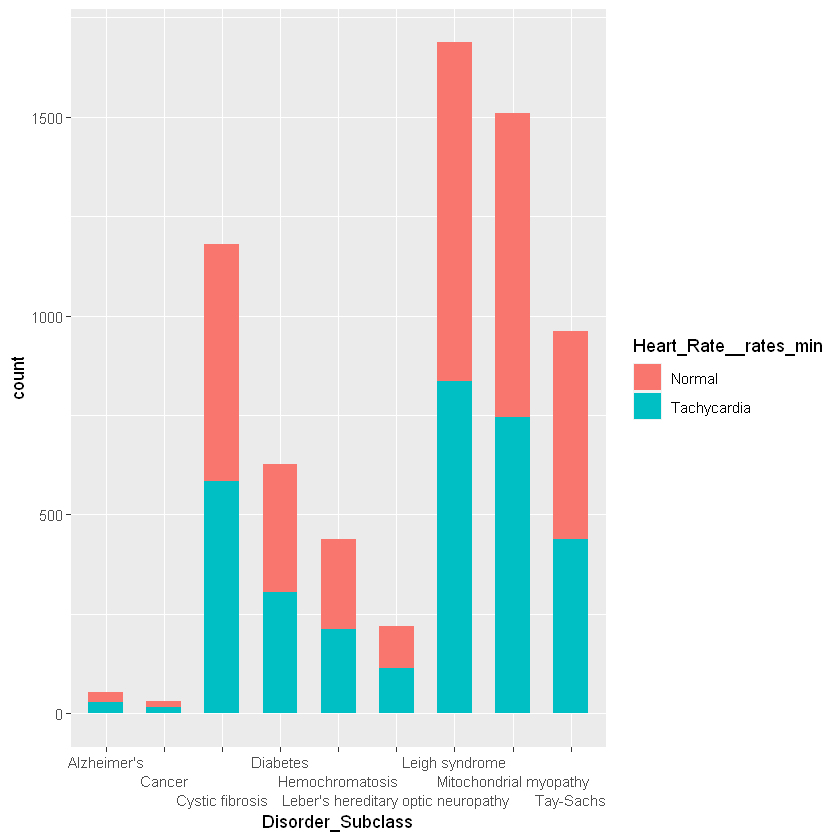
\includegraphics[height=10cm, width=12cm]{figures/heartrate.png}
	\caption{Disorder And Heart - rate}
	\label{fig 6}
\end{figure}

\begin{figure}[htpb]
	\centering
	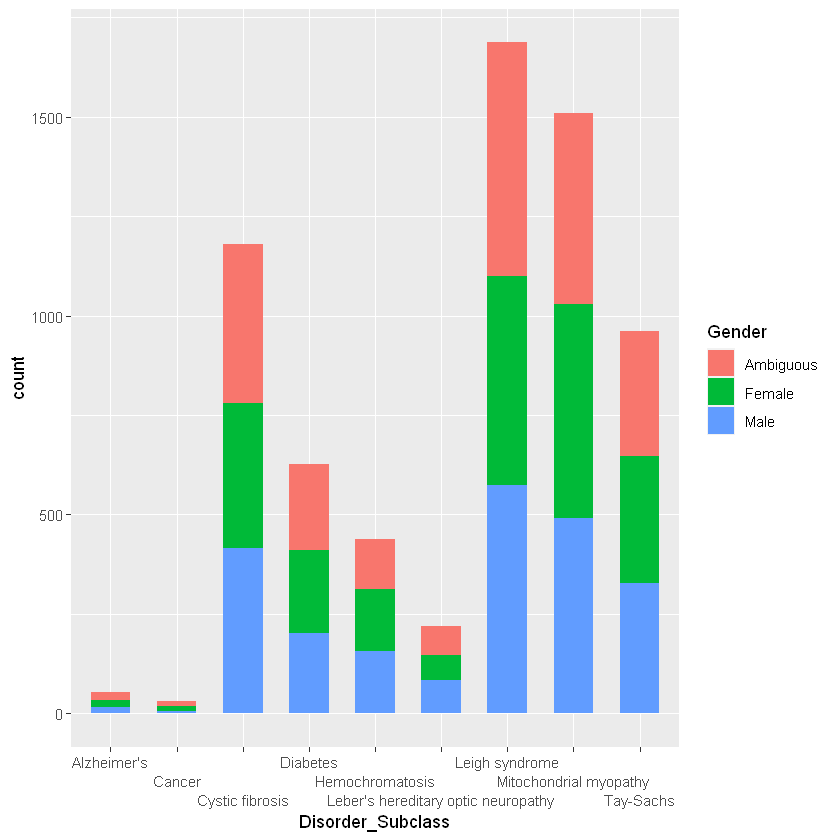
\includegraphics[height=10cm, width=12cm]{figures/gender.png}
	\caption{Disorder And Gender}
	\label{fig 7}
\end{figure}

\begin{figure}[htpb]
	\centering
	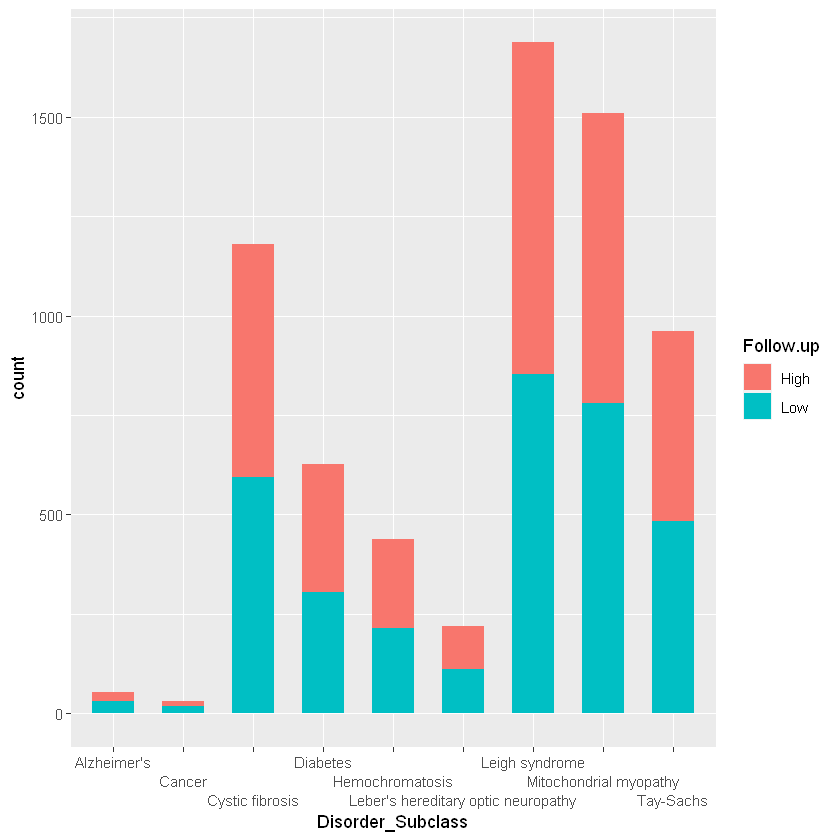
\includegraphics[height=10cm, width=12cm]{figures/follow.png}
	\caption{Disorder And Follow up}
	\label{fig 8}
\end{figure}

\begin{figure}[htpb]
	\centering
	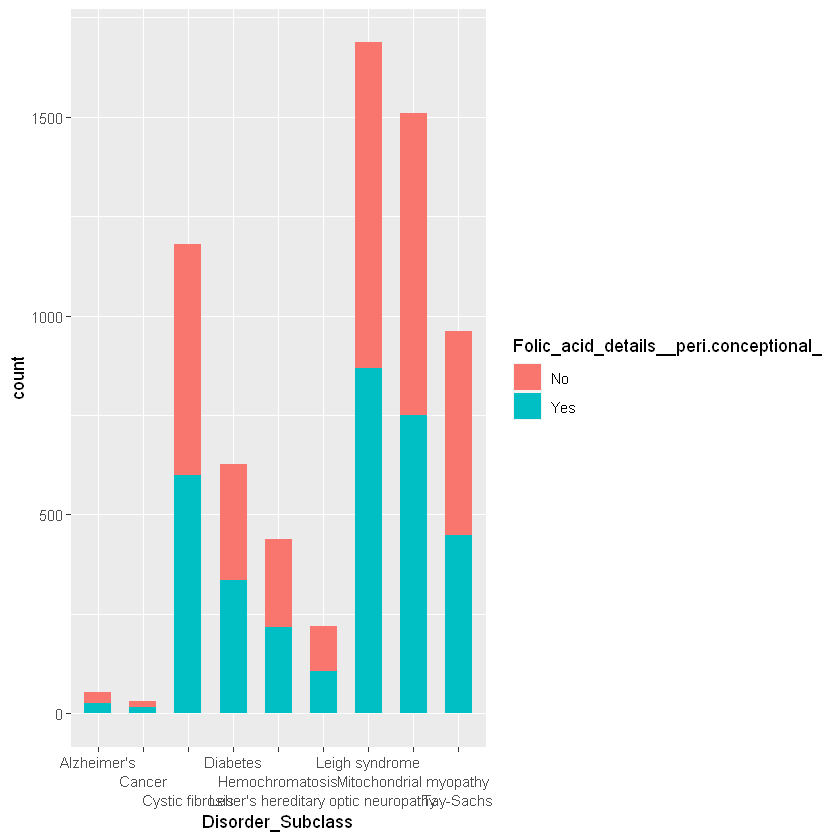
\includegraphics[height=10cm, width=12cm]{figures/folicacid.png}
	\caption{Disorder And Folic Acid details}
	\label{fig 9}
\end{figure}

\begin{figure}[htpb]
	\centering
	\includegraphics[height=10cm, width=12cm]{figures/Blood.png}
	\caption{Disorder And Blood Test Result}
	\label{fig 10}
\end{figure}

\begin{figure}[htpb]
	\centering
	\includegraphics[height=10cm, width=12cm]{figures/Birthdefect.png}
	\caption{Disorder And Birth Defect}
	\label{fig 11}
\end{figure}

\begin{figure}[htpb]
	\centering
	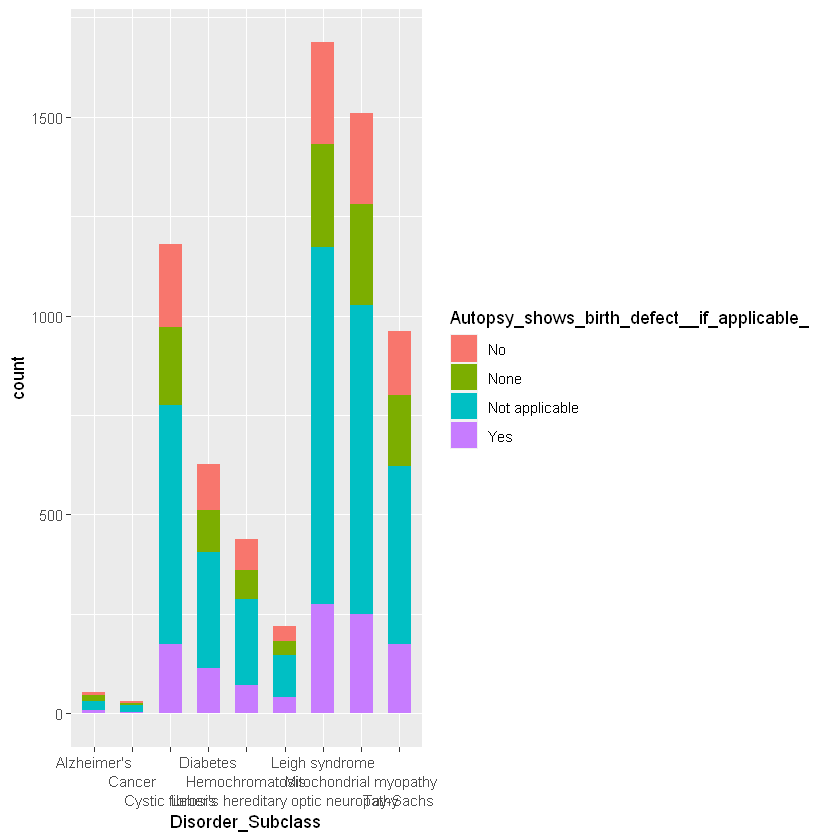
\includegraphics[height=10cm, width=12cm]{figures/autopsy.png}
	\caption{Disorder And Autopsy Report}
	\label{fig 12}
\end{figure}

\begin{figure}[htpb]
	\centering
	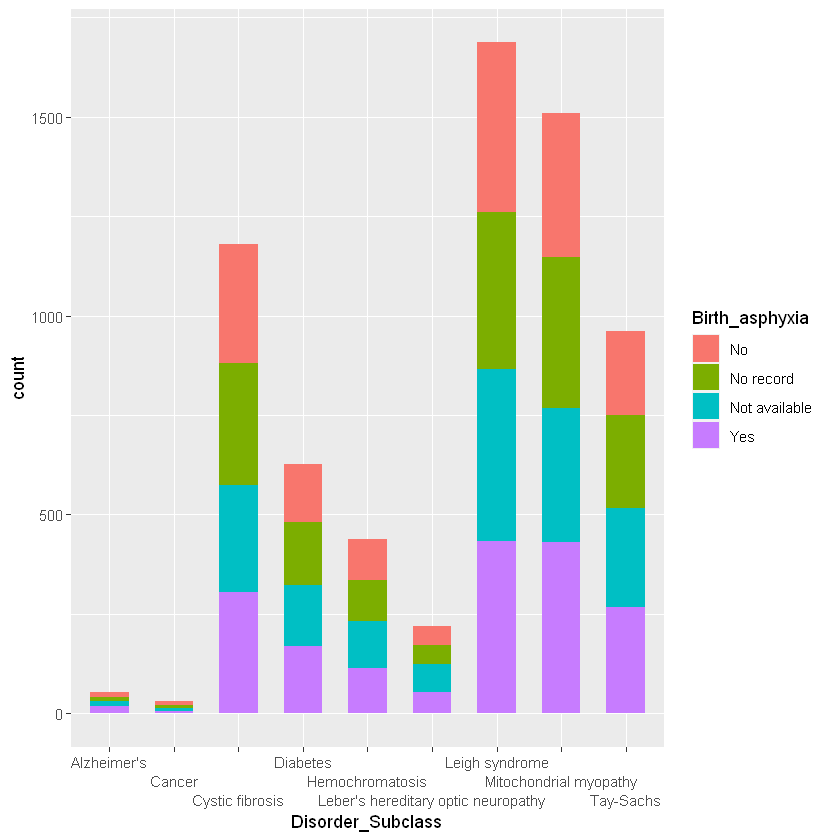
\includegraphics[height=10cm, width=12cm]{figures/asphyxia.png}
	\caption{Disorder And Asphyxia}
	\label{fig 13}
\end{figure}

\begin{figure}[htpb]
	\centering
	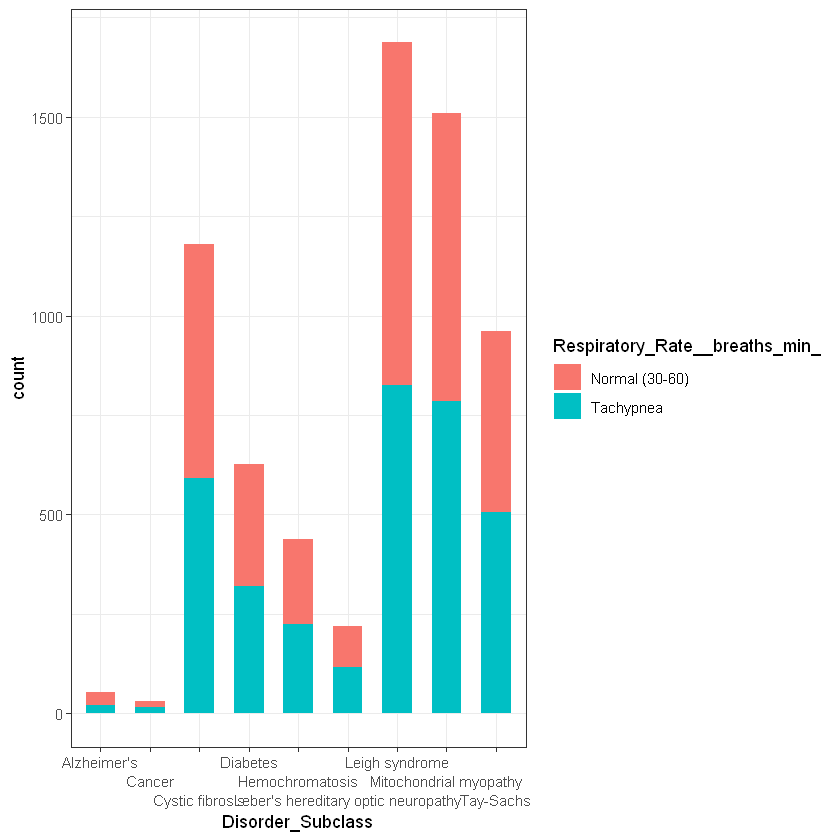
\includegraphics[height=10cm, width=12cm]{figures/resp.png}
	\caption{Disorder And Respiratory Rate}
	\label{fig 14}
\end{figure}

\begin{figure}[htpb]
	\centering
	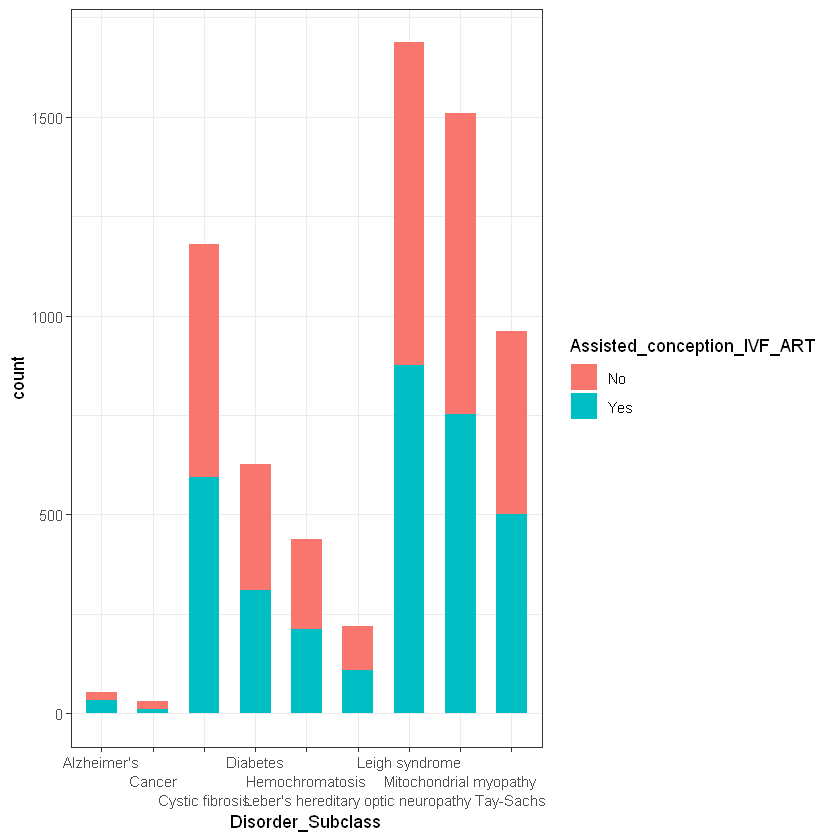
\includegraphics[height=10cm, width=12cm]{figures/ivf.png}
	\caption{Disorder And IVF details}
	\label{fig 15}
\end{figure}
\begin{figure}[htpb]
	\centering
	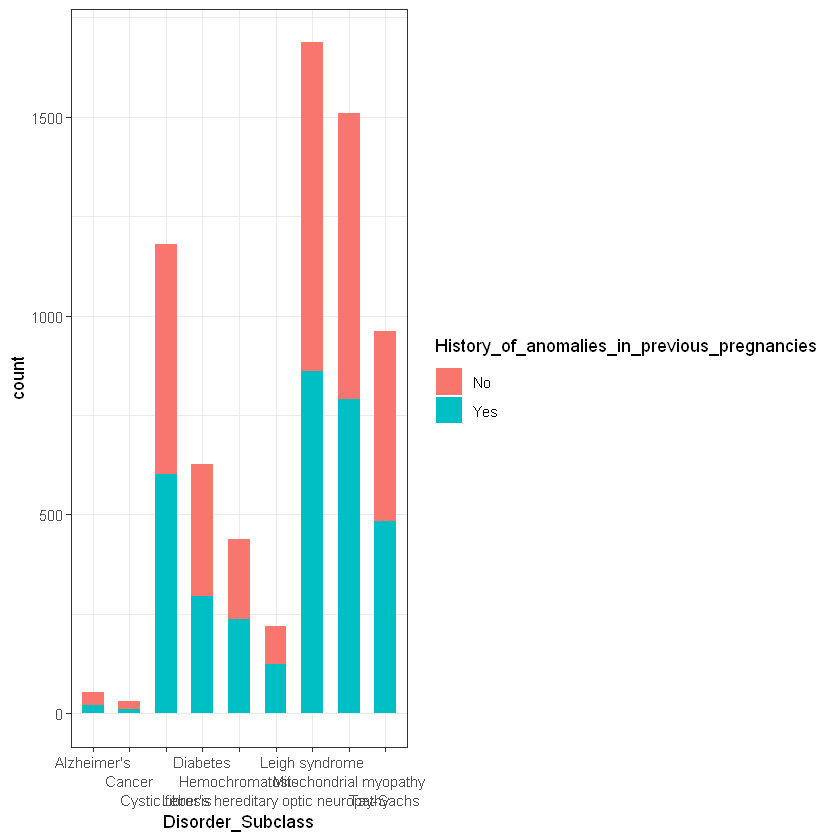
\includegraphics[height=10cm, width=12cm]{figures/preg.png}
	\caption{Disorder And History Of Pregnancy}
	\label{fig 16}
\end{figure}
\newpage
\noindent
We also found fully dependent relation between the two target attributes. That is, The Genetic Disorder attribute can be derived from the Disorder Subclass attribute. Hence that can also be now removed.
\begin{figure}[htpb]
	\centering
	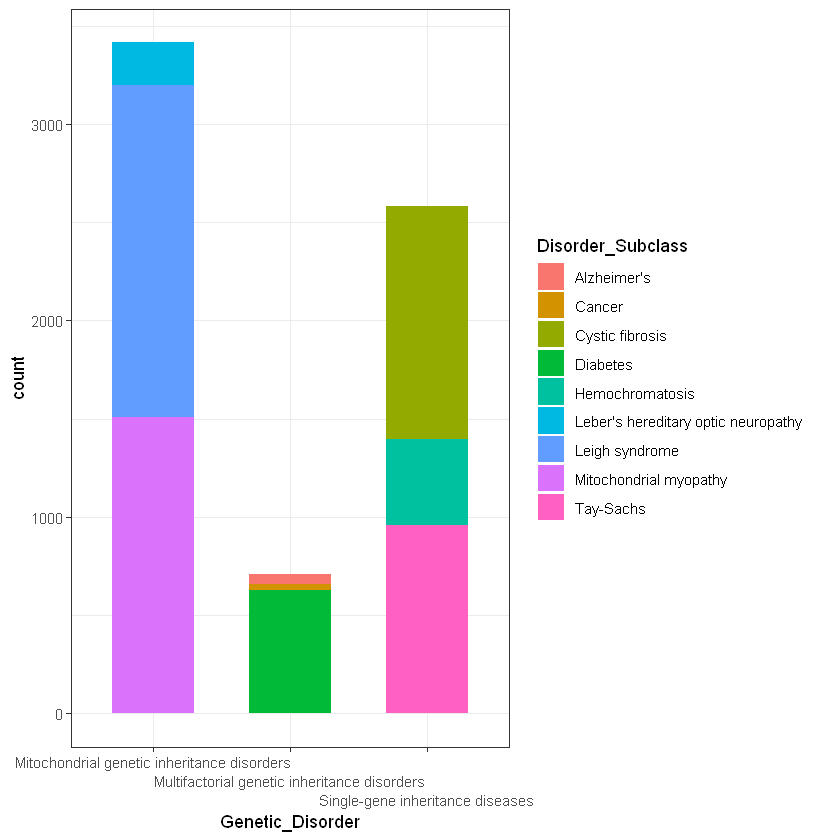
\includegraphics[height=10cm, width=12cm]{figures/rel.png}
	\caption{Relation Between Target Attributes }
	\label{fig 17}
\end{figure}
\paragraph{}

\noindent
\noindent
For the Numeric attributes, a disorder-wise Box and Whisker plots were created and it displayed relatively significant variance in one or more disorder.


\begin{figure}[htpb]
	\centering
	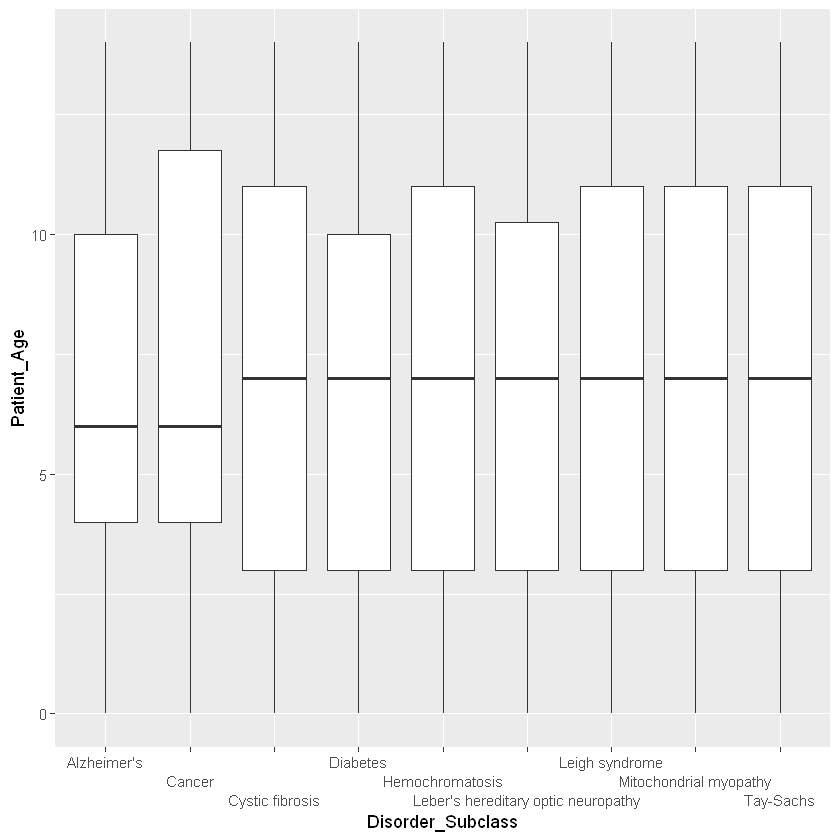
\includegraphics[height=10cm, width=12cm]{figures/p-age.png}
	\caption{Disorder And Patient's Age}
	\label{fig 18}
\end{figure}

\begin{figure}[htpb]
	\centering
	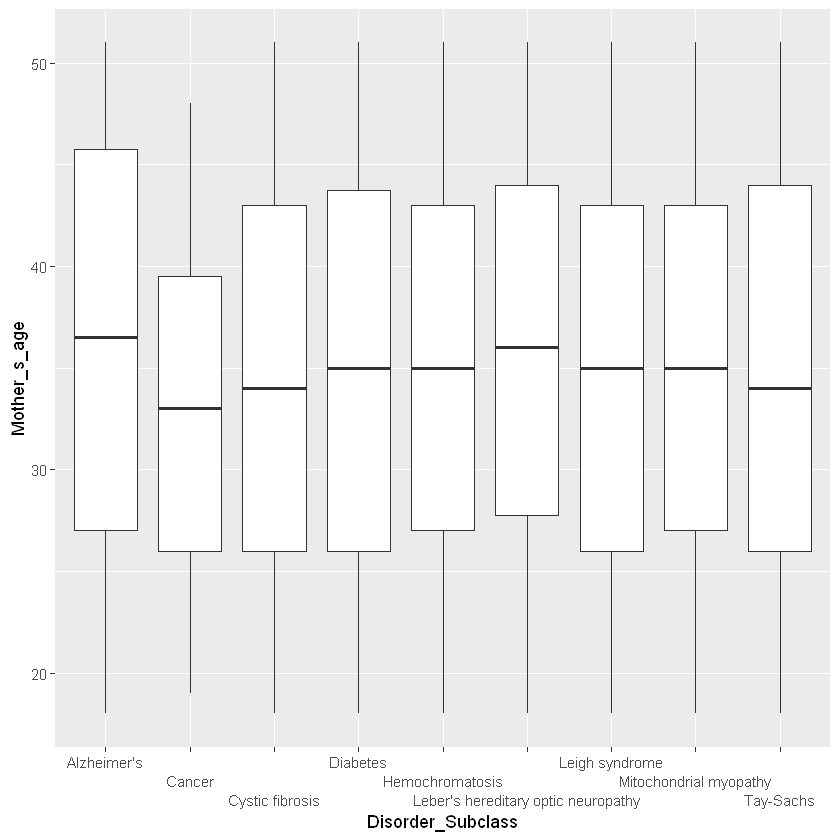
\includegraphics[height=10cm, width=12cm]{figures/m-age.png}
	\caption{Disorder And Patient's Mother's Age }
	\label{fig 19}
\end{figure}
\begin{figure}[htpb]
	\centering
	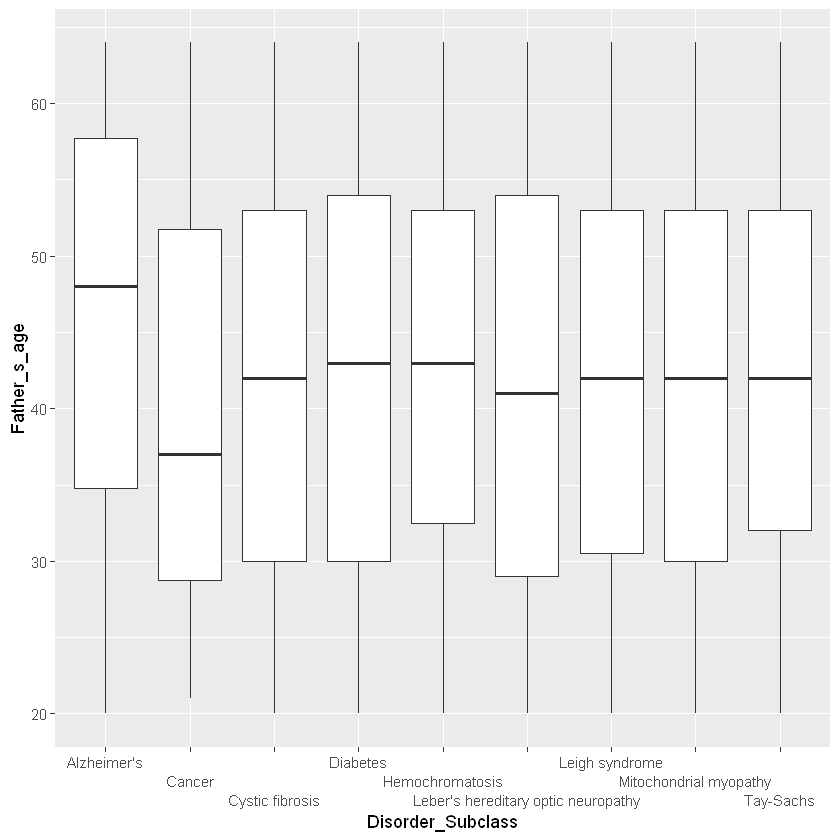
\includegraphics[height=10cm, width=12cm]{figures/f-age.png}
	\caption{Disorder And Patient's Father's Age }
	\label{fig 20}
\end{figure}
\begin{figure}[htpb]
	\centering
	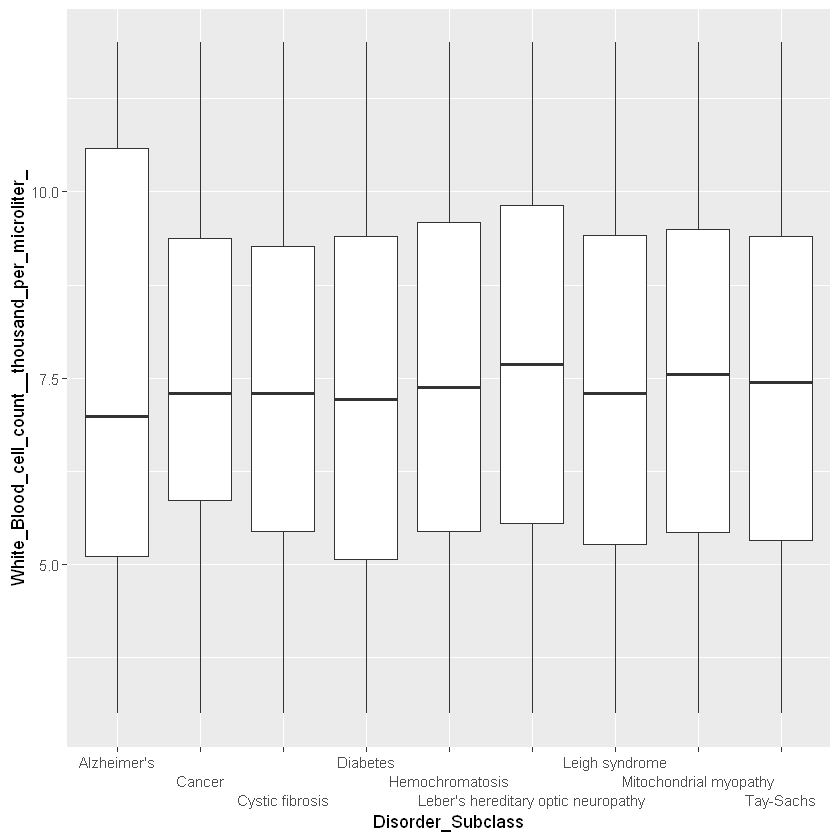
\includegraphics[height=10cm, width=12cm]{figures/wbc.png}
	\caption{Disorder And White Blood Cell Count}
	\label{fig 21}
\end{figure}
\begin{figure}[htpb]
	\centering
	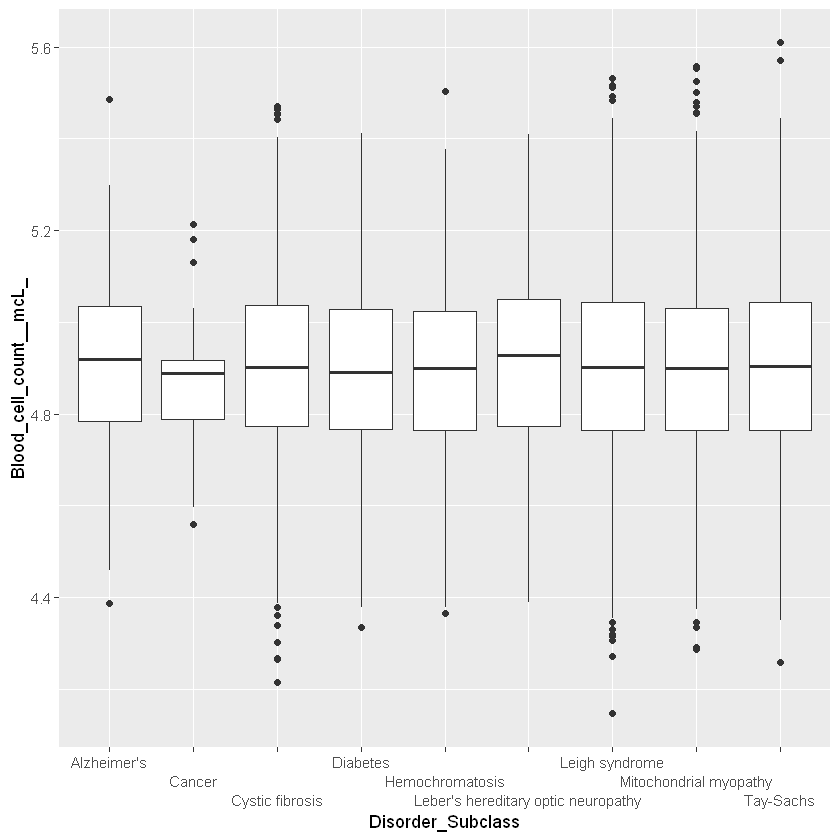
\includegraphics[height=10cm, width=12cm]{figures/bc.png}
	\caption{Disorder And Blood Cell Count}
	\label{fig 22}
\end{figure}
\begin{figure}[htpb]
	\centering
	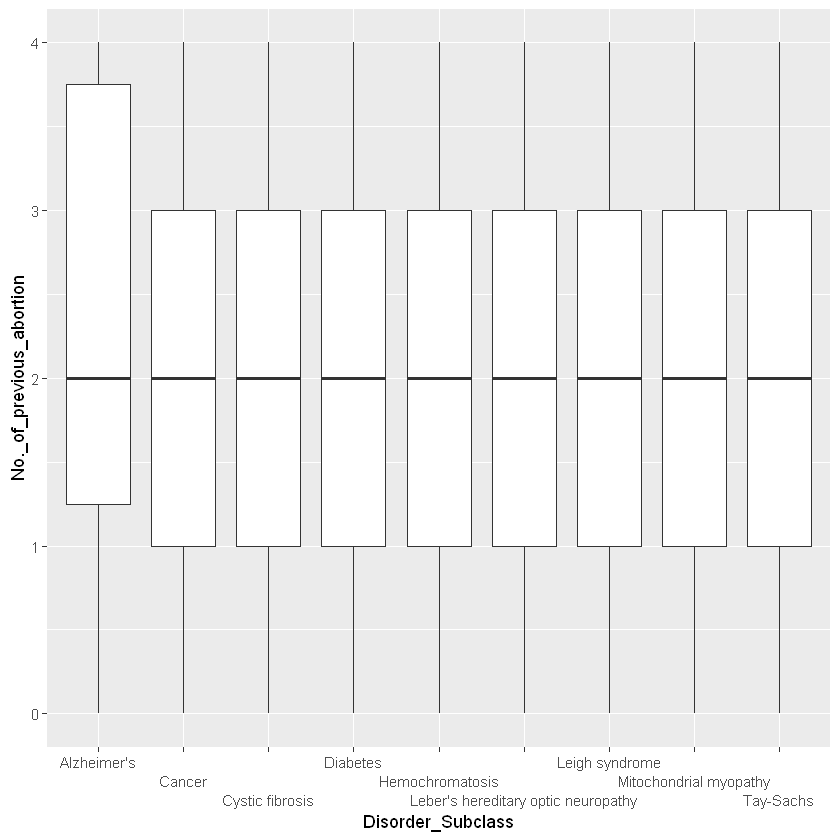
\includegraphics[height=10cm, width=12cm]{figures/npa.png}
	\caption{Disorder And Number Of Previous Abortions}
	\label{fig 23}
\end{figure}
\newpage
 \noindent
Based on the domain expertise the following columns are considered significant and have shown a good variance as such can prove proper information to classify the disorder on future data.
\begin{figure}[htpb]
	\centering
	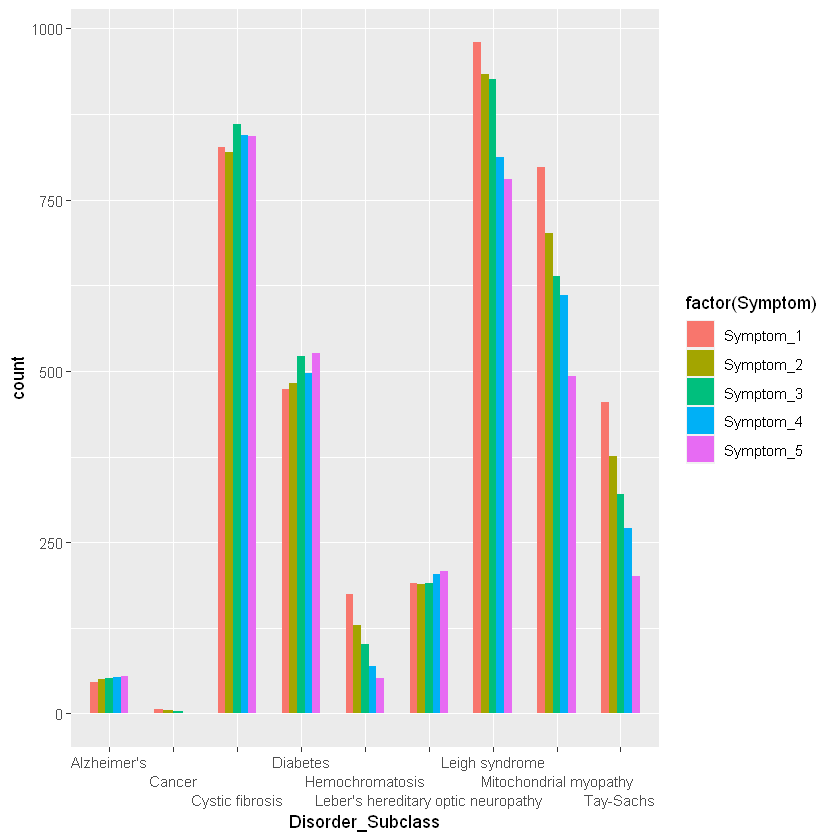
\includegraphics[height=8cm, width=10cm]{figures/s1.png}
	\caption{Disorder And Frequency Of Symptoms Being True}
	\label{fig 24}
\end{figure}
\begin{figure}[htpb]
	\centering
	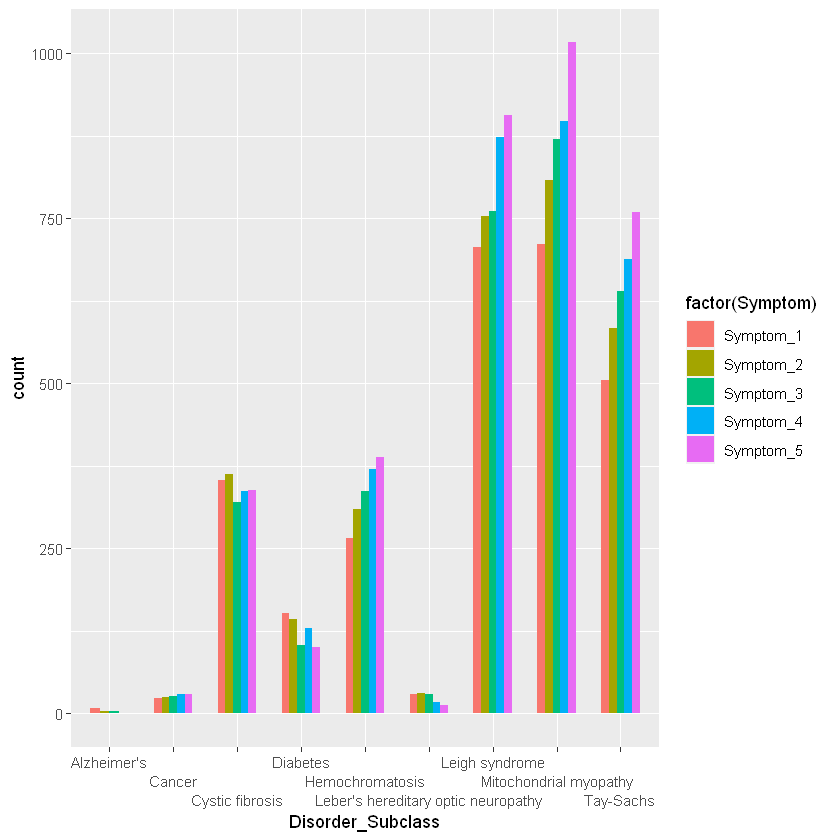
\includegraphics[height=8cm, width=10cm]{figures/s0.png}
	\caption{Disorder And Frequency Of Symptom Being False}
	\label{fig 25}
\end{figure}
\begin{figure}[htpb]
	\centering
	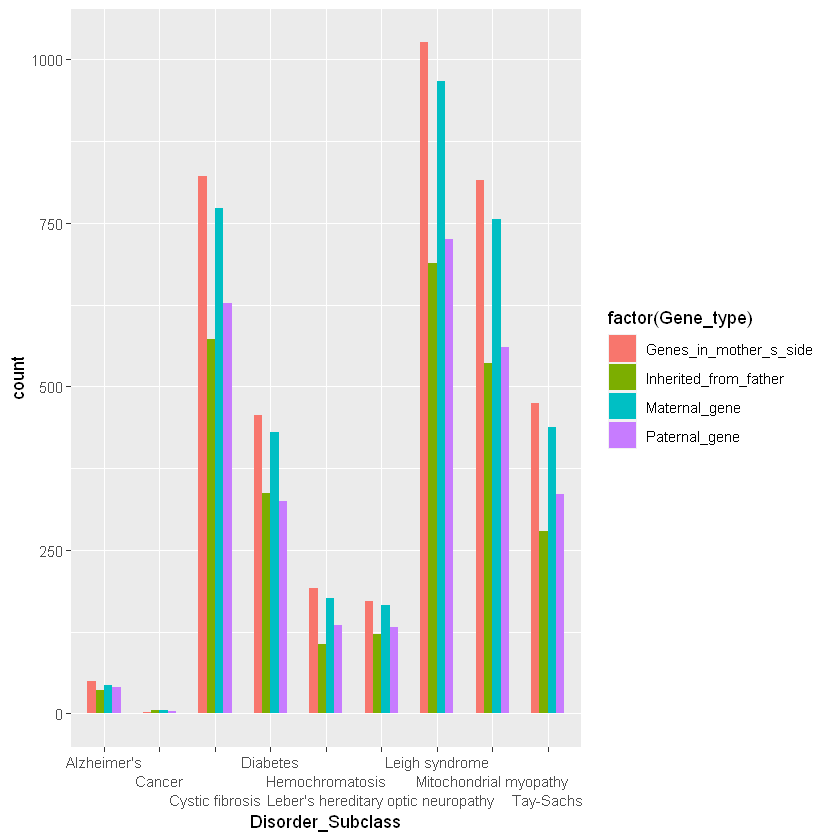
\includegraphics[height=10cm, width=12cm]{figures/gy.png}
	\caption{Disorder And Frequency Of Gene Being Yes}
	\label{fig 26}
\end{figure}
\begin{figure}[htpb]
	\centering
	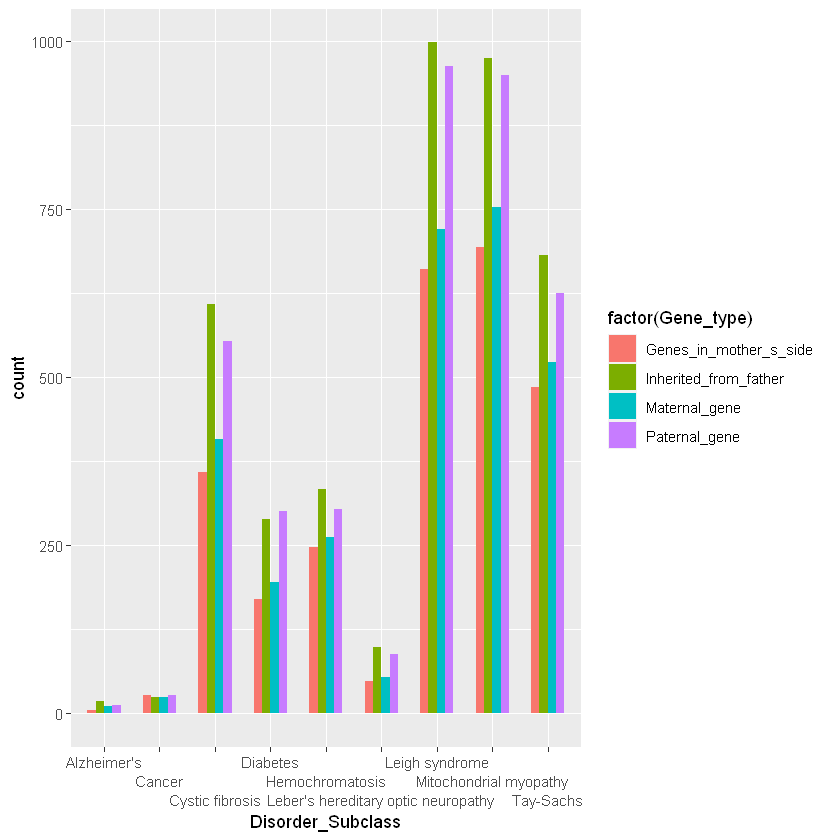
\includegraphics[height=10cm, width=12cm]{figures/gn.png}
	\caption{Disorder And Frequency Of Gene Being No}
	\label{fig 27}
\end{figure}
\newpage
\section{Dashboard}
Also an interactive dashboard is implemented using \url{https://visual.is} which can be found in \url{https://visual.is/visualizations/new-visualization/bpqD6MZM9CzQb8UTKZUThdx4}.\\
\begin{figure}[htpb]
	\centering
	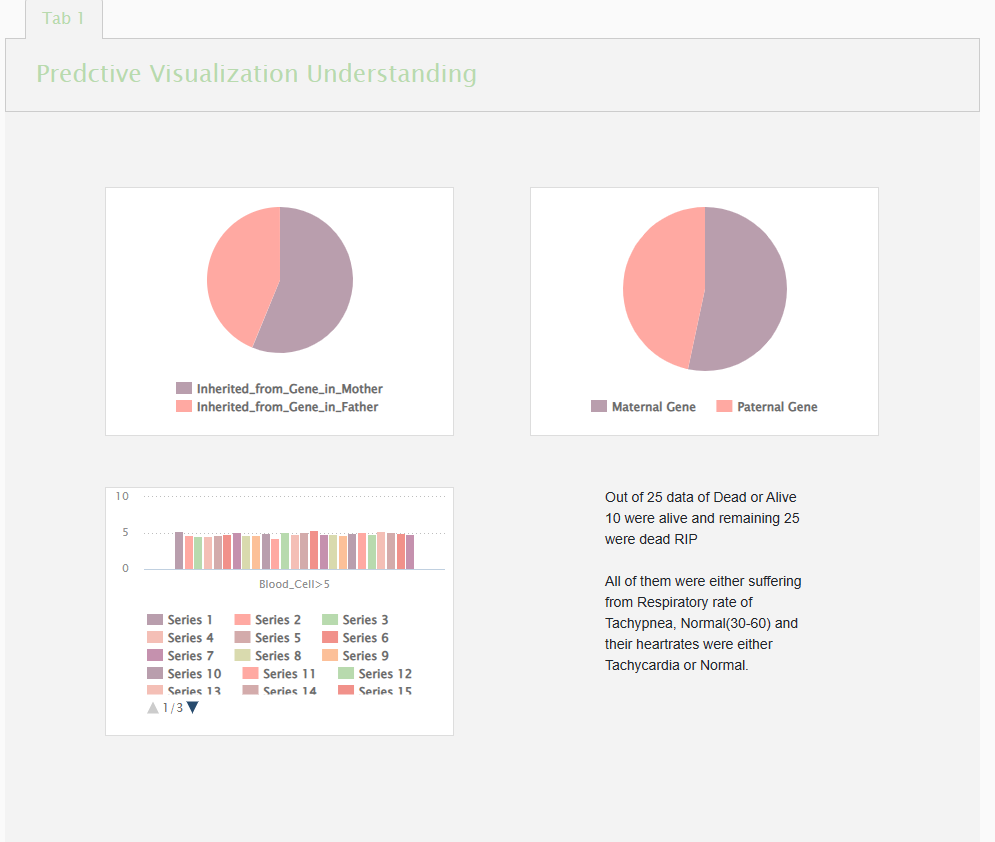
\includegraphics[height=10cm, width=12cm]{figures/dash.png}
	\caption{Dashboard Sample}
	\label{fig 28}
\end{figure}
\newpage

\chapter{CONCLUSIONS}

In this EDA project, we aimed to gain insights and streamline the dataset by applying various techniques including statistical analysis, graphical visualization, and domain knowledge. Our objective was to reduce the dimensionality of the dataset while retaining important and informative features. Through a comprehensive analysis, we successfully reduced the dataset from 45 columns to 16 columns.
\begin{table}[htpb]
	\caption{Remaining Columns}
	\centering
	\begin{tabular}{|l|}
		\hline
		Patient Age\\
		Genes in mother's side\\
		Inherited from father\\
		Maternal gene\\
		Paternal gene\\
		Blood cell count mcL\\
		Mother's age\\
		Father's age\\
		Number of previous abortion\\
		White Blood cell count thousand per microliter\\
		Symptom 1 \\
		Symptom 2\\
		Symptom 3\\
		Symptom 4\\
		Symptom 5 \\                          
		Disorder Subclass\\ 
		\hline
	\end{tabular}
	\label{tab 2}
\end{table}
\newline
\noindent
Statistical analysis played a crucial role in identifying key features that significantly contributed to the dataset. By evaluating statistical measures such as mean, standard deviation, and correlation coefficients, we were able to quantify the relationships between variables and make informed decisions on feature selection.\\
\noindent
Graphical visualization techniques were employed to visualize patterns, trends, and outliers in the data. Box plots, scatter plots, and histograms provided valuable insights into the distribution and relationships of variables. By visually examining the data, we gained a deeper understanding of its characteristics, which guided us in selecting the most relevant features.\\
\noindent
Domain knowledge also played a significant role in feature selection. By leveraging our understanding of the subject matter, we were able to identify domain-specific attributes that were essential for analysis and decision-making. This domain-based information added an additional layer of context and relevance to the feature selection process.\\
\noindent
Our approach was further supported by citable sources, including research papers that discuss the importance of feature selection, dimensionality reduction, and the impact of domain knowledge in data analysis. These sources provided a theoretical foundation and best practices for our EDA project.\\
\noindent
Additionally, we implemented a dashboard to present the analyzed data in a visually appealing and interactive manner. The dashboard allowed users to explore the reduced dataset, visualize trends, and gain actionable insights efficiently. By incorporating user-friendly features and interactive elements, the dashboard facilitated data-driven decision-making and enhanced the overall user experience.\\
\noindent
In conclusion, our EDA project successfully reduced the dataset from 45 columns to 16 columns through the application of statistical analysis, graphical visualization, and domain-based information. The feature selection process was supported by citable sources, ensuring the validity and reliability of our approach. The implementation of a dashboard provided an effective means of visualizing the analyzed data and empowered users to make informed decisions based on the insights gained.\\ 
\noindent
Future work could involve further refinement of the feature selection process, exploration of advanced visualization techniques, and integration of machine learning algorithms for predictive modeling based on the reduced dataset.







%=====================================================================
% For Reference settings
%%%%%%%%%%%%%%%%%%%%%%%%%%%%%%%%%%%%%%%%%%%%%%%%%%%%%%%%%%%%%%%%%%%%%
\renewcommand{\bibname}{\centering REFERENCES}
\bibliographystyle{amsplain}

\bibliography{bibtex_database/myrefs} % data base
%===================================================================
\end{document}
